\definition
For $\alpha > 0$, consider also the following variant $\mathrm{LWE}_{q, \leq \alpha}$ of worst case LWE: For any $s \in \Z_q^n$ and any (unknown) $\beta \leq \alpha$, given samples from $A_{s, \Psi_\beta}$, retrieve $s$.

\proposition{Unknown to constant error variance reduction}
\label{lwe_leq_alpha_lwe_alpha}
Given an oracle for worst case LWE with error distribution $\Psi_\alpha$, we can solve $\mathrm{LWE}_{q, \leq \alpha}$.

\begin{proof}
The idea of this proof is the following lemma from \cite[2.2]{Reg}:
\paragraph{Lemma} For any $\alpha > 0$ and $0 < \epsilon \leq \alpha$, we have that the statistical distance between $\Psi_\alpha$ and $\Psi_{\alpha + \epsilon}$ is at most $9\epsilon / \alpha$.
\\\\
Let $p(n) \in (0, 1]$ be the success probability of the oracle and $m \in O(\mathrm{poly}(n))$ the amount of samples the oracle needs. Then define 
\begin{equation}
\epsilon := \frac 1 {18m} p \alpha \quad \text{ and } \quad N = \alpha/\epsilon \in O(\mathrm{poly}(n)) \nonumber
\end{equation}
Given samples $(A, b) \sim A_{s, \beta}$ we can now find $s$ by calling the oracle on $(A, b + e_k)$ for each $k \in \{ 0, ..., N \}$, where $e_k \sim \nu_{k\epsilon}^m$ is a normal random variable. If one of these calls returns the correct secret (we can check that), this is our result. We have to show that with high probability, this happens. 

Let $k$ be the smallest number with $k\epsilon \geq \alpha - \beta$. We claim that with high probability, the oracle returns the correct secret when called on $(A, b + e_k)$. The random variable $(A, b + e_k)$ is distributed like $A_{s, \Psi_{\beta + k\epsilon}}$, and by the lemma, the statistical distance to $A_{s, \Psi_\alpha}$ is at most $9\epsilon / \alpha$. Therefore, the statistical distance between $A_{s, \Psi_{\beta + k\epsilon}}^m$ and $A_{s, \Psi_\alpha}^m$ is at most $m 9\epsilon / \alpha = \frac 1 2 p$. Since applying the oracle cannot increase the statistical distance, the output of the oracle on $(A, b + e_k)$ is within distance $\frac 1 2 p$ of the output on valid samples $(A', b') \sim A_{s, \Psi_\alpha}^m$, and therefore, we find the secret with probability at least $\frac 1 2 p$. \qedhere
\end{proof}

\theorem{SIVP to LWE reduction}
\label{hardness_lwe}
For $\alpha q \geq 2\sqrt{n}$, there is a quantum reduction from worst case $\mathrm{LWE}_{q, \leq \alpha}$ to worst case $\mathrm{SIVP}_{2n\sqrt{2n}/\alpha}$. Using some stronger bounds on $\eta_\epsilon(L)$, \cite{Reg} even proves the reduction to  $\mathrm{SIVP}_{2n\sqrt{2\omega(\log(n))}/\alpha}$.

\subsection{Remark}
We will present a summary of the proof given in \cite{Reg}. This proof relies heavily on some technical results about the smoothing parameter and the discrete gaussian distribution that go beyond the scope of this work. Therefore, we will only sketch some edge parts of the argument, but we try to present the main ideas formally correct (namely the use of the LWE oracle and the quantum part of the reduction).

\begin{proof}
The heart of the proof is the following lemma:

\lemma[Improvement of gaussian samples using LWE]
\label{recursive_step}
Let $\epsilon$ be negligible, $\alpha \in (0, 1)$ and $r > \sqrt{2}q\eta_\epsilon(L)$. Given an oracle for $\mathrm{LWE}_{q, \leq \alpha}$ and samples from $D_{L, r}$ (as many as the oracle needs), we can efficiently generate samples from $D_{L, r\sqrt{n}/\alpha q}$. The generated samples are stochastically independent of the input samples and of each other.

\begin{proof}
We begin with stating the following lemma on the inner product with discrete gaussian vectors:
\paragraph{Lemma 1}
For a lattice $L,\ z, u \in \R^n,\ r, \alpha > 0$ and $\epsilon \leq \frac 1 2$ with 
\begin{equation}
1 / \sqrt{\frac 1 {r^2} + \frac {\| z \|^2} {\alpha^2}} \geq \eta_{\epsilon}(L) \nonumber
\end{equation}
we have for random variables $v \sim D_{L + u, r}$ and $e$ normally distributed with standard deviation $\alpha/\sqrt{2\pi}$ that the $\langle z, v \rangle + e$ is within statistical distance $4\epsilon$ to
\begin{equation}
\nu_{\sqrt{(r\| z \|)^2 + \alpha^2}} \nonumber
\end{equation}
In particular, we get that $\langle z, qv \rangle + qe \mod q$ is within statistical distance $4\epsilon$ to $\Psi_\alpha$.

\begin{proof} \noqed See e.g. \cite[3.10]{Reg}. 
    
    Intuitively, this lemma says that the scalar product of a constant vector with a vector drawn from the discrete gaussian distribution is distributed like an LWE error.
\end{proof}

Let $L = \mathcal{L}(B)$ and $L^* = \mathcal{L}(B^*)$ with $B^* = \left(B^{-1}\right)^T$. For this proof, we also require a variant of the BDD problem:
\subsection{Definition $\mathrm{BDD}_{L, \gamma}^q$}
Define the problem as: Given $x \in \R^n$ close to $L$, calculate the coefficients of $\kappa(x)$ modulo $q$, i.e.\ calculate $s \mod q$ where $Bs = \kappa(x)$ when given a point $x$ close to $L$ (within distance $\gamma$)
\\\\
Then proof consists of the following parts:
\begin{itemize}
\item Construct an oracle for $\mathrm{BDD}_{L^*, \alpha q / \sqrt{2}r}^q$.
\item Construct an oracle for $\mathrm{BDD}_{L^*, \alpha q / \sqrt{2}r}$.
\item Using this, quantumly generate samples from $D_{L, r\sqrt{n}/\alpha q}$.
\end{itemize}

\subsection{Oracle for $\mathrm{BDD}_{L^*, \alpha q / \sqrt{2}r}^q$}
Let $v_1, ..., v_n \in L$ denote the samples from $D_{L, r}$, so have $v_1, ..., v_n$ iid. random variables with $v_i \sim D_{L, r}$. On input $x \in \R^n$ with $\| x - \kappa(x) \| \leq \alpha q / r\sqrt{2}$ define
\begin{equation}
\begin{split}
s = \left(B^*\right)^{-1} \kappa(x) = B^T \kappa(x) &\in \Z^n \quad \text{ since } \quad \kappa(x) \in L^* \\
a_i = B^{-1} v_i &\in \Z^n \nonumber
\end{split}
\end{equation}
and get
\begin{equation}
\langle a_i, s \rangle = \langle B^{-1}v_i, B^T \kappa(x) \rangle = \langle v_i, \kappa(x) \rangle = \langle v_i, x \rangle + \langle v_i, \kappa(x) - x \rangle \nonumber
\end{equation}
The statistical distance between $a_i \mod q$ and a uniform random variable on $\Z_q^n$ is negligible by \ref{smoothing_parameter_smooth_discrete_structure}.
Now we condition on a fixed $a_i \mod q$. We get that $v_i / q \sim D_{L + Ba_i / q, r / q}$ and
\begin{equation}
1 / \sqrt{\frac {q^2} {r^2} + 2\frac {\| \kappa(x) - x \|^2} {\alpha^2}} \geq 1 / \sqrt{\frac {q^2} {r^2} + 2 \frac {\alpha^2 q^2} {\alpha^2 2 r^2} } = \frac r {\sqrt{2}q} > \eta_\epsilon(L) \nonumber
\end{equation}
so we can apply lemma 1 with $u = Ba_i / q$ and get that $\langle v_i / q, \kappa(x) - x \rangle + e$ is distributed according to $\nu_\beta$ where $e \sim \nu_{\alpha / \sqrt{2}}$ is a normal random variable with standard deviation $\alpha / 2\sqrt{\pi}$ and $\beta^2 = (r\| x - \kappa(x) \| / q)^2 + (\alpha/\sqrt{2})^2 \leq \alpha^2$. Since this holds conditioned on any arbitrary $a_i$, the error random variable $\langle v_i / q, \kappa(x) - x \rangle + e$ is also independent from $a_i$. Therefore, $(a_i \mod q, \langle v_i, x \rangle + qe \mod q)$ are valid samples of $A_{s, \Psi_\beta}$ and our oracle can retrieve $s \mod q$.

\subsection{Oracle for $\mathrm{BDD}_{L^*, \alpha q / \sqrt{2}r}$}
The idea is to find the digits of the coefficients in the base $q$ by repeatedly applying the oracle to new points. Let $x \in \R^n$ with $\| x - \kappa(x) \| \leq \alpha q/\sqrt{2}r$ be the input. Denote by $s$ the coefficients of $\kappa(x)$, i.e. $s = B^T \kappa(x)$. Now define
\begin{equation}
\begin{split}
x_0 &= x \\
x_{i + 1} &= \frac {x_i - B (s_i \mod q)} q \\
s_{i} &= \left\lfloor \frac s {q^i} \right\rfloor = \frac {s - (s \mod q^i)} {q^i} \in \Z^n \nonumber
\end{split}
\end{equation}
Then $\kappa(x_i) = Bs_i$ by induction, since for $x'_i = x_i - B (s_i \mod q)$ we get $x'_i - x_i = B (s_i \mod q) \in L$ so
\begin{equation}
\kappa(x'_i)  = \kappa(x_i) - B(s_i \mod q) = B\left(s_i - (s_i \mod q)\right) = B q \left\lfloor \frac s {q^{i + 1}} \right\rfloor = Bqs_{i + 1} \nonumber
\end{equation}
Since $\| a - \kappa_\Lambda(a) \| \leq \| a - \kappa_\Gamma(a) \|$ if $\Gamma$ is a sublattice of $\Lambda$, we get $\kappa_{qL}(x'_i) = Bqs_{i+1}$ and therefore
\begin{equation}
\kappa(x_{i + 1}) = \kappa_L\left(\frac {x'_i} q\right)  = \kappa(x_{i + 1}) = Bs_{i + 1} \nonumber
\end{equation}
Using this and the oracle, we can also calculate $x_{i + 1}$ and so $(s_{i + 1} \mod q)$ given $x_i$ and $s_i \mod q$. By repeating this, we get $s_i \mod q$ for any $i$. Now we find $s$ by using that $s = \sum_i s_i \mod q$.

\subsection{Generate sample of $D_{L, r\sqrt{n}/\alpha q}$}
\paragraph{Overview} Some readers might not be used to quantum computation, so an elaborate high-level overview about this part will be presented before we come to the technical details.
The main idea is that the (continous) fourier transformation transforms a distribution of repeated wide gaussians on the dual lattice to a distribution of the wanted (narrow) discrete gaussian on $L$. With ``distribution of repeated gaussians'' we mean the distribution resulting from choosing a lattice point and adding some (continous) gaussian noise, see figure \ref{repeated_gaussians}.
\begin{figure}[ht]
\centering
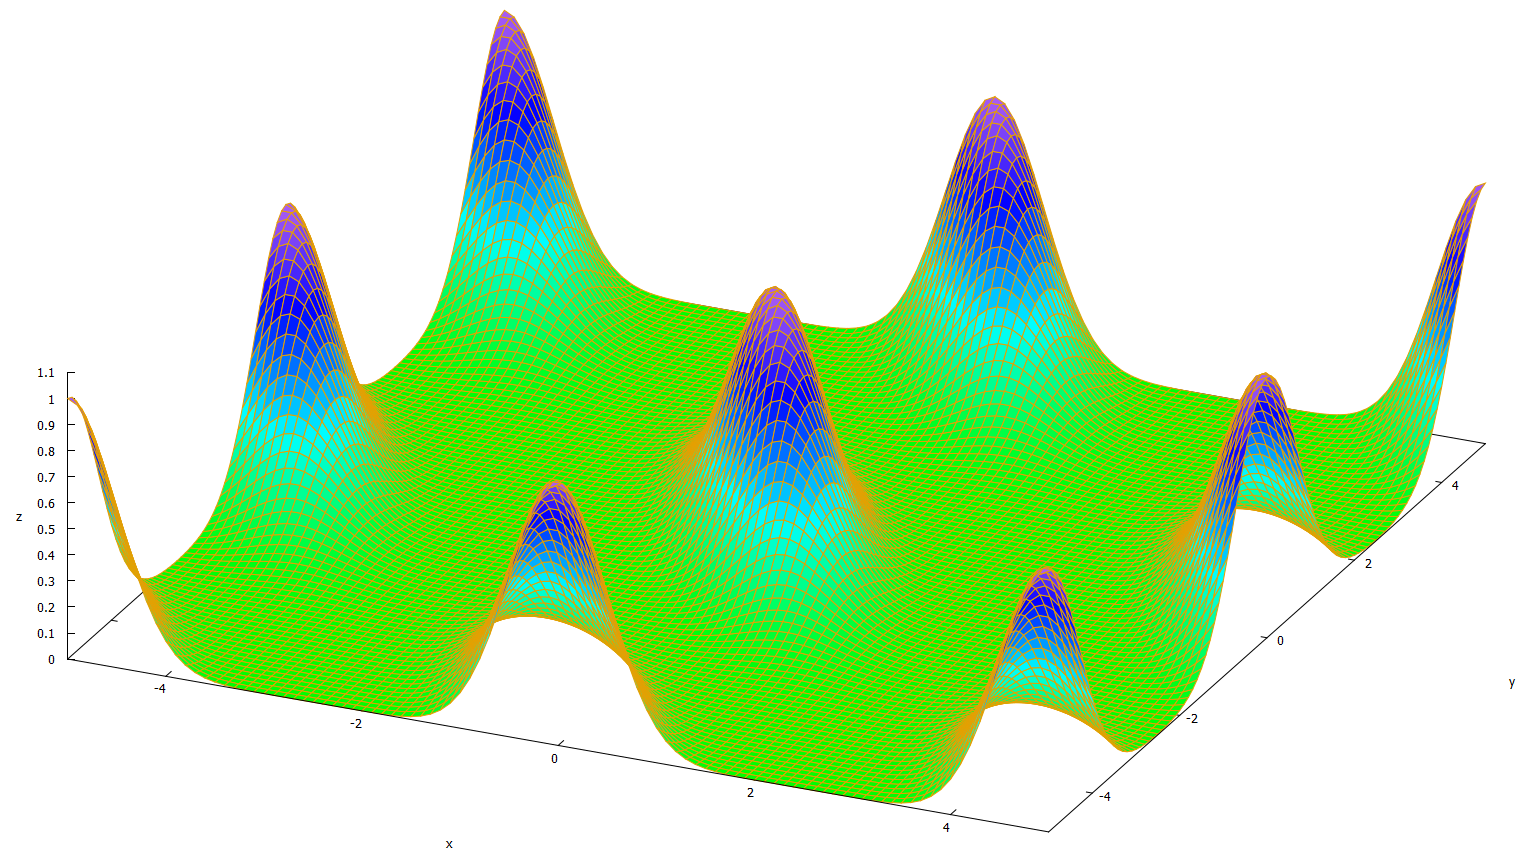
\includegraphics[width=\textwidth]{repeated_gaussians.png}
\caption{Inverse fourier transform of $D_{L, r}$, the ``repeated gaussians''}
\label{repeated_gaussians}
\end{figure}
Therefore, we can approximate the discrete gaussians on $L$ by applying the discrete fourier transformation on an approximation of this source distribution. Classically, this is of no use as we require exponentially many points to represent the source distribution well enough. However, the quantum fourier transform allows us to process exponentially many points in polynomial time, given a suitable superposition of them, something like
\begin{equation}
\sum_{x \in \R^n} e^{-\mathrm{dist}(x, L)^2} |x\rangle \nonumber
\end{equation}
Of course, we cannot sum over $\R$. In reality, we will use all points on a fine grid within the fundamental parallelepiped. Creating this state is not easy however, due to a caveat inherent to quantum computation. The first step of the ``sample lattice points and add noise'' still works, leading to a state that looks like
\begin{equation}
\sum_{x \in \R^n} e^{-\|x - \kappa(x) \|^2} |x\rangle \otimes |\kappa(x)\rangle \nonumber
\end{equation}
There is one problem in this equation though. The qbits containing the noisy point $|x\rangle$ are entangled with the original lattice point we added the noise to, namely $|\kappa(x)\rangle$. In quantum mechanics, all operations have to be reversible, so we cannot just ``drop'' the unwanted qbits without destroying the superposition we need. But since we can compute $|\kappa(x)\rangle$ from $|x\rangle$ using the BDD-oracle, we can ``uncompute'' the $|\kappa(x)\rangle$ part by applying the quantum gates of the oracle in reverse  and get the required superposition.

\paragraph{Details}
Let  $d =\alpha q/ r\sqrt{2n}$ and $R = 2^{3n}d\lambda_n(L^*)\sqrt{n}$ be a big enough integer (representing the fine grid size). Then we claim that the effect of the QFT can be described by
\begin{equation}
\QFT \sum_{x \in \frac 1 R L^*} \rho_d(x) \left|x \mod \mathcal{P}(B^*)\right\rangle = \det(RB) \sum_{t \in L} \rho_{1/d}(t) \left|t \mod \mathcal{P}(RB)\right\rangle \label{eq_result_qft}
\end{equation}
where $\mathcal{P}(B)$ is the fundamental parallelepiped generated by the basis vectors in $B$. When we consider the limit $R \to \infty$, this corresponds to the abstract idea presented earlier, as the left part becomes an integral and the $t \mod \mathcal{P}(RB)$ becomes $t$. We have
\begin{equation}
\begin{split}
&\QFT \sum_{x \in \frac 1 R L^*} \rho_d(x) \left|x \mod \mathcal{P}(B^*)\right\rangle \\
=& \ \QFT \sum_{x \in \frac 1 R L^* \cap \mathcal{P}(B^*)} \rho_d(x + L^*) \left|x\right\rangle \\
=& \ \sum_{t \in L \cap \mathcal{P}(RB)} \ \sum_{x \in \frac 1 R L^* \cap \mathcal{P}(B^*)} \exp(-2\pi i \langle x, t \rangle) \rho_d(x + L^*) \left|t\right\rangle \\
=& \ \sum_{t \in L \cap \mathcal{P}(RB)} \ \sum_{x \in \frac 1 R L^*} \exp(-2\pi i \langle x, t \rangle) \rho_d(x) \left|t\right\rangle \\
=& \det(RB)  \sum_{t \in L \cap \mathcal{P}(RB)} \ \sum_{x \in RL} \rho_{1/d}(x - t) \left|t\right\rangle \\
=& \det(RB) \sum_{t \in L} \rho_{1/d}(t) \left|t \mod \mathcal{P}(RB)\right\rangle \nonumber
\end{split}
\end{equation}
where the second-last line holds due to the Poisson summation formula (Since $\rho$ is equal to its fourier transformation, so $\rho_d = \hat\rho_{1/d}$). Here the use of the QFT on lattices should be the natural extension from the QFT on the coefficients, i.e.
\begin{equation}
\begin{split}
&\QFT \sum_{x \in \frac 1 R L \cap \mathcal{P}(B)} f(x) \left|x\right\rangle = \QFT \sum_{z \in \Z_R^n} f\left(\frac {Bz} R \right) \left|\frac {Bz} R \right\rangle \\
:=& \sum_{k \in \Z_R^n} \ \sum_{z \in \Z_R^n} f\left(\frac {Bz} R \right) \exp\left(-2\pi i\frac {\langle k, z \rangle} R\right) \left|B^* k\right\rangle \\
=& \sum_{k \in \Z_R^n} \ \sum_{x \in \frac 1 R L \cap \mathcal{P}(B)} f(x) \exp\left(-2\pi i \langle k, B^{-1}x \rangle \right) \left|B^* k\right\rangle \\
=& \sum_{k \in \Z_R^n} \ \sum_{x \in \frac 1 R L \cap \mathcal{P}(B)} f(x) \exp\left(-2\pi i \langle B^*k, x \rangle \right) \left|B^* k\right\rangle \\
=& \sum_{y \in L^* \cap \mathcal{P}(RB^*) } \ \sum_{x \in \frac 1 R L \cap \mathcal{P}(B)} f(x) \exp\left(-2\pi i \langle y, x \rangle \right) \left|y\right\rangle \nonumber
\end{split}
\end{equation}
This transform can be done by a quantum computer in polynomial time by multiplying the input register with $RB^{-1}$, then applying the standard QFT and then multiplying the result with $B^*$.

Note that the second term in the QFT result shown above (equation \ref{eq_result_qft}) is almost exactly what we want: When we measure this state, we get $t \mod \mathcal{P}(RB)$ for a $t$ chosen from $D_{L, 1/d\sqrt{2}}$ (since the probability of getting $t$ is proportional to $\rho_{1/d}(t)^2 = \rho_{1/d\sqrt{2}}(t)$). By the following lemma, we can efficiently get $t$ from $t \mod \mathcal{P}(RB)$, and therefore get a sample from $D_{L, 1/d\sqrt{2}} = D_{L, r\sqrt{n}/\alpha q}$. 

We can use the lemma, since $\lambda_1(RL) = R\lambda_1(L) \geq 2^{3n}d\sqrt{n}$ by using $\lambda_n(L^*)\lambda_1(L) \geq 1$ (by \ref{gaussian_length_bound}). In particular, $\lambda_1(RL) \geq d\sqrt{2n}$ and solving $\mathrm{BDD}_{RL, d\sqrt{n}/\sqrt{2}}$ is equivalent to solving $\mathrm{BDD}_{L, d\sqrt{n}/R\sqrt{2}}$ which is possible in polynomial time because $d\sqrt{n}/R\sqrt{2}$ is exponentially small (e.g. by using Babai's nearest plane algorithm).

\paragraph{Lemma 2}
Let $L = \mathcal{L}(B)$ be a lattice, $c > 0$ and $x \sim D_{L/c, \gamma}$ be a random variable with $\lambda_1(L) \geq 2\gamma\sqrt{n}$ and define $x' := x \mod \mathcal{P}(B)$. Assume we have access to an oracle for $\mathrm{BDD}_{L, \gamma\sqrt{n}}$. Then we can efficiently calculate $x$ given $x' = x \mod \mathcal{P}(B)$ with probability of at least $1 - 2^{-2n}$.

\begin{proof}
By \ref{gaussian_length_bound}, the probability that $\|x\| < \gamma\sqrt{n}$ is at least $1 - 2^{-2n}$. If this is the case, we have that $\| x - \kappa(x) \| < \gamma\sqrt{n}$, and so $\|\kappa(x') - x'\| < \gamma\sqrt{n}$. By using the oracle, we can calculate $\kappa(x')$.

Now we use that $\lambda_1(L) \geq 2\gamma\sqrt{n}$. This yields that $\kappa(x) = 0$, since the distance between the lattice points $0$ and $\kappa(x)$ is $< 2\gamma\sqrt{n} \leq \lambda_1(L)$. Similarly, we have $\kappa(x) - \kappa(x') = x - x'$, because the distance between the lattice points  $\kappa(x) - \kappa(x')$ and $x - x'$ is
\begin{equation}
\| \kappa(x) - \kappa(x') - x + x' \| \leq \| \kappa(x) - x \| + \| \kappa(x') - x' \| < 2\gamma\sqrt{n} \leq \lambda_1(L) \nonumber
\end{equation}
Therefore we find $x$ by $x = x' + \kappa(x) - \kappa(x') = x' - \kappa(x')$.

The intuition in this argument is that $x$ is distributed very narrowly around the origin. Therefore, $x \mod \mathcal{P}(B)$ is very close to one of the corners of the fundamental parallelepiped, and the location of $x \mod \mathcal{P}(RB)$ relative to this corner is the location of $x$ relative to the origin. \qedhere
\end{proof}

\paragraph{Creating the initial state} 
We have shown that we can get a sample from the right side of equation \ref{eq_result_qft}, so it remains to be shown that we can efficiently create the state on the left side, namely
\begin{equation}
\sum_{x \in \frac 1 R L^*} \rho_d(x) |x \mod \mathcal{P}(B^*)\rangle \nonumber
\end{equation}
It is not obvious, but this state corresponds to the ``repeated gaussian'' distribution mentioned earlier: Taking the gaussian (almost continous for large $R$) modulo the fundamental parallelepiped yields a distribution in which there are ``hills'' in each corner of the parallelepiped, and by filling the complete space with copies of the parallelepiped, we get the ``repeated gaussian'' distribution.

By dividing the register by $R$, we can easily get this state when we start with the state
\begin{equation}
\sum_{x \in L^*} \rho_{Rd}(x) |x \mod \mathcal{P}(RB^*)\rangle \nonumber
\end{equation}
As shown in \cite{Reg} 3.2, we can efficiently create the state
\begin{equation}
\sum_{x \in L^*} \rho_{Rd}(x) |x\rangle \nonumber
\end{equation}
Classically, it looks like we could just take this state modulo $\mathcal{P}(RB^*)$ and be done. The problem is that quantum operations have to be reversible, so we have to be able to calculate $x$ from $x \mod \mathcal{P}(RB^*)$ in order to do this. Luckily, we can do that using Lemma 2:

We have $\lambda_1(RL^*) = R\lambda_1(L^*) \geq 2Rd\sqrt{n}$ since
\begin{equation}
2d\sqrt{n} = \frac {\alpha q} {r \sqrt{2}} \leq \frac {\alpha q} {2q\eta_\epsilon(L)} = \frac \alpha {2\eta_\epsilon(L)} \leq \frac 1 {2\eta_\epsilon(L)} \leq \frac {\lambda_1(L)} 2 \nonumber
\end{equation}
where the last inequality follows from \ref{smoothing_parameter_lower_bound} and we can solve $\mathrm{BDD}_{RL^*, Rd\sqrt{n}}$ which is equivalent to $\mathrm{BDD}_{L^*, d\sqrt{n}} = \mathrm{BDD}_{L^*, \alpha q/r\sqrt{2}}$ by using the oracle constructed earlier. \qedhere
\end{proof}

\paragraph{Proof of \ref{hardness_lwe}}
The idea is to start with samples of a very wide gaussian distribution which are easy to generate, and then improve them using the lemma \ref{recursive_step} above. This way, we can get samples of a very narrow gaussian distribution. Among $n^2$ of these are $n$ linearly independent one with very high probability, so we can use them to solve SIVP.

\subparagraph{Show} For a given $r \geq n \sqrt{2}\lambda_n(L)/\alpha$ we can efficiently sample from $D_{L, r}$. \\
As shown in \cite{Reg}, we can efficiently sample from $D_{L, r'}$ for some computable, exponentially large $2^{3n}\lambda_n(L) \geq r' \geq 2^{2n} \lambda_n(L)$. The idea in that argument is to use a LLL basis of $L$. Let $\epsilon = 2^{-n}$ and apply lemma \ref{recursive_step} repeatedly on these samples to create shorter ones. The condition of \ref{recursive_step} is fullfilled as long as the input radius is $\geq q \sqrt{2n} \lambda_n(L)$, because by \ref{smoothing_parameter_upper_bound} and \ref{lambda_dual_lattice} we have
\begin{equation}
\sqrt{2}q\eta_\epsilon(L) \leq \frac {q \sqrt{2n}} {\lambda_1(L^*)} \leq q \sqrt{2n} \lambda_n(L) \nonumber
\end{equation}
Therefore we can reach the given $r$ by repeated applications, because we have by assumption that $r \geq n\sqrt{2}\lambda_n(L)/\alpha \geq q \sqrt{2n} \lambda_n(L) \sqrt{n}/\alpha q$.
Since every application of the recursive step shrinks the radius by a factor of $2$, we can get samples of $D_{L, r}$ through polynomially many repetitions (as $\log r'/r$ is polynomial in $n$).

\paragraph{Lemma 3} The probability that $n^2$ independent samples of $D_{L, r}$ for some $r \geq \sqrt{2}\eta_\epsilon(L)$ are contained in any $n-1$ dimensional hyperplane is exponentially small. In other words, the probability that there are $n$ linearly independent samples among those $n^2$ ones is exponentially close to $1$.

\begin{proof} \noqed
See \cite[3.16]{Reg}.
\end{proof}

Now it looks like we could just get $n^2$ samples from $D_{L, r}$ for $r = n\sqrt{2}\lambda_n(L)/\alpha$ and output $n$ linearly independent ones from among them (they have length $\leq 2n\sqrt{n}\lambda_n(L)/\alpha$ by \ref{gaussian_length_bound}). The only problem however is that we do not know $\lambda_n(L)$, so we cannot give the right $r$ to the sampling oracle. We can however apply the whole procedure for each $r_k = 2^{-k}r' n\sqrt{2}/\alpha$ where $r'$ is the exponential upper bound for $\lambda_n(L)$ mentioned above and take the shortest set of independent samples we find. Since $2^{3n}\lambda_n(L) \geq r' \geq 2^{2n} \lambda_n(L)$, there must be some $k \in \{ 2n, ..., 3n \}$ so that 
\begin{equation}
r_k = 2^{-k} r' n\sqrt{2}/\alpha \in \left[n \sqrt{2}\lambda_n(L)/\alpha, 2n \sqrt{2}\lambda_n(L)/\alpha \right] \nonumber
\end{equation}
So when we try that $k$, we sample $n^2$ vectors from $D_{L, r_k}$ and find $n$ linearly independent vectors of length $\leq 2n \sqrt{2n}\lambda_n(L)/\alpha$ with high probability, which solves $\mathrm{SIVP}_{2n\sqrt{2n}/\alpha}$. \qedhere
\end{proof}










